\definecolor{Red}{RGB}{217,33,32}
\definecolor{Blue}{RGB}{63,96,174}
\definecolor{Duck}{RGB}{83,158,182}
\definecolor{Green}{RGB}{109,179,136}
\definecolor{Yellow}{RGB}{202,184,67}
\definecolor{Orange}{RGB}{231,133,50}
\definecolor{Red}{RGB}{217,33,32}
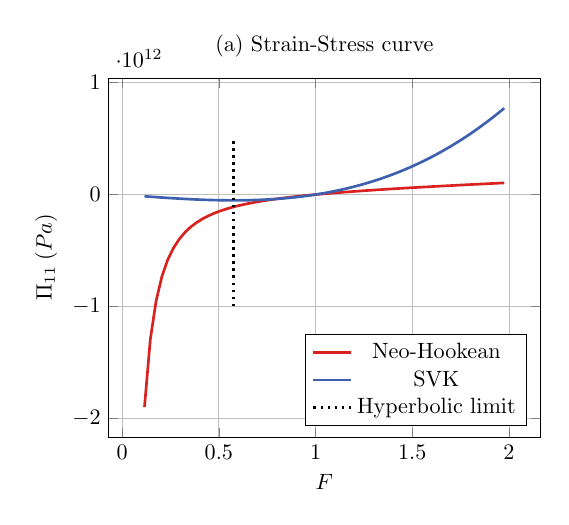
\begin{tikzpicture}[scale=0.8]
\begin{axis}[xlabel=$F$,ylabel=$\Pi_{11} \: (Pa)$,ymajorgrids=true,xmajorgrids=true,legend pos=south east,title={(a) Strain-Stress curve}]
\addplot[Red,very thick] coordinates {(0.11547005383792518,-1898966453319.162) (0.14547005383792516,-1296837707486.0405) (0.17547005383792513,-951312235719.5623) (0.20547005383792513,-732355105152.6451) (0.23547005383792513,-583575852118.2125) (0.2654700538379251,-477087968993.8754) (0.2954700538379251,-397729449724.4541) (0.3254700538379251,-336642141070.28204) (0.35547005383792507,-288349957545.72546) (0.38547005383792504,-249309520683.61847) (0.415470053837925,-217140040714.9308) (0.44547005383792504,-190190468824.5224) (0.475470053837925,-167284549773.97247) (0.505470053837925,-147564580724.34894) (0.535470053837925,-130392343185.27245) (0.5654700538379249,-115284401045.16144) (0.595470053837925,-101868733030.67676) (0.625470053837925,-89854990617.66492) (0.6554700538379249,-79013679521.07468) (0.6854700538379249,-69161318053.14328) (0.7154700538379248,-60149680216.69014) (0.7454700538379249,-51857881714.88495) (0.7754700538379249,-44186477584.150566) (0.8054700538379248,-37053004869.531456) (0.8354700538379248,-30388577783.986546) (0.8654700538379249,-24135259235.847366) (0.8954700538379248,-18244011798.887867) (0.9254700538379248,-12673085866.843775) (0.9554700538379248,-7386740998.494719) (0.9854700538379247,-2354223588.251995) (1.0154700538379247,2451056537.9352818) (1.0454700538379247,7052193879.264957) (1.0754700538379247,11469332294.041113) (1.1054700538379247,15720112571.176903) (1.1354700538379248,19820042073.450085) (1.1654700538379246,23782801671.8228) (1.1954700538379246,27620501912.14364) (1.2254700538379246,31343897846.142628) (1.2554700538379246,34962570023.63762) (1.2854700538379247,38485077640.53793) (1.3154700538379245,41919088663.206696) (1.3454700538379245,45271490826.59238) (1.3754700538379245,48548486673.378265) (1.4054700538379246,51755675220.64049) (1.4354700538379246,54898122376.10795) (1.4654700538379246,57980421852.87309) (1.4954700538379244,61006748029.95563) (1.5254700538379244,63980901961.52675) (1.5554700538379245,66906351538.24785) (1.5854700538379245,69786266641.0072) (1.6154700538379245,72623549993.23035) (1.6454700538379243,75420864307.28705) (1.6754700538379244,78180656228.87244) (1.7054700538379244,80905177507.05946) (1.7354700538379244,83596503754.174) (1.7654700538379244,86256551106.45828) (1.7954700538379245,88887091051.8295) (1.8254700538379243,91489763653.42323) (1.8554700538379243,94066089365.83081) (1.8854700538379243,96617479614.0105) (1.9154700538379243,99145246281.97147) (1.9454700538379244,101650610238.83322) (1.9754700538379242,104134709013.2085) };
\addplot[Blue,very thick] coordinates {(0.11547005383792518,-15336791766.165447) (0.14547005383792516,-19168111304.289738) (0.17547005383792513,-22893685303.277996) (0.20547005383792513,-26491706070.822536) (0.23547005383792513,-29940365914.61566) (0.2654700538379251,-33217857142.349674) (0.2954700538379251,-36302372061.71689) (0.3254700538379251,-39172102980.40962) (0.35547005383792507,-41805242206.12016) (0.38547005383792504,-44179982046.540825) (0.415470053837925,-46274514809.36392) (0.44547005383792504,-48067032802.28176) (0.475470053837925,-49535728332.98665) (0.505470053837925,-50658793709.17089) (0.535470053837925,-51414421238.526794) (0.5654700538379249,-51780803228.74666) (0.595470053837925,-51736131987.522804) (0.625470053837925,-51258599822.54755) (0.6554700538379249,-50326399041.513176) (0.6854700538379249,-48917721952.112) (0.7154700538379248,-47010760862.036354) (0.7454700538379249,-44583708078.97849) (0.7754700538379249,-41614755910.630775) (0.8054700538379248,-38082096664.68549) (0.8354700538379248,-33963922648.83495) (0.8654700538379249,-29238426170.77144) (0.8954700538379248,-23883799538.187305) (0.9254700538379248,-17878235058.774815) (0.9554700538379248,-11199925040.226295) (0.9854700538379247,-3827061790.2340784) (1.0154700538379247,4262162383.5095387) (1.0454700538379247,13089555173.312326) (1.0754700538379247,22676924271.481888) (1.1054700538379247,33046077370.32594) (1.1354700538379248,44218822162.15218) (1.1654700538379246,56216966339.268196) (1.1954700538379246,69062317593.98189) (1.2254700538379246,82776683618.60081) (1.2554700538379246,97381872105.43274) (1.2854700538379247,112899690746.78526) (1.3154700538379245,129351947234.96603) (1.3454700538379245,146760449262.28293) (1.3754700538379245,165147004521.04358) (1.4054700538379246,184533420703.55563) (1.4354700538379246,204941505502.12674) (1.4654700538379246,226393066609.06476) (1.4954700538379244,248909911716.677) (1.5254700538379244,272513848517.2716) (1.5554700538379245,297226684703.1562) (1.5854700538379245,323070227966.6382) (1.6154700538379245,350066286000.0256) (1.6454700538379243,378236666495.6256) (1.6754700538379244,407603177145.7466) (1.7054700538379244,438187625642.6959) (1.7354700538379244,470011819678.7812) (1.7654700538379244,503097566946.3102) (1.7954700538379245,537466675137.5906) (1.8254700538379243,573140951944.9299) (1.8554700538379243,610142205060.6364) (1.8854700538379243,648492242177.0171) (1.9154700538379243,688212870986.3801) (1.9454700538379244,729325899181.0331) (1.9754700538379242,771853134453.2832) };
\addplot[dotted,very thick] coordinates {(sqrt(1./3.),-1.e12) (sqrt(1./3.),0.5e12)};
\legend{Neo-Hookean,SVK,Hyperbolic limit}
\end{axis}
\end{tikzpicture}
